One of the simplest partial differential equations that exhibits
spatiotemporal chaotic behavior is the \KS\ [henceforth KS]
system\rf{KurTsu76, siv}, which is used to model a number of different
phenomena, such as unstable flame fronts. The equation for the velocity
of such a flame front
$u(\conf, \zeit)$ on a periodic domain, $u(\conf, \zeit)= u(\conf + L,
\zeit)$.
\beq
    u_\zeit + \frac{1}{2}(u^2)_\conf + u_{\conf \conf} + \nu u_{\conf \conf \conf \conf} = 0 \, \quad x \in [0, L]
\eeq
The terms each contribute differently to the dynamics: $u_{\conf \conf}$
contributes to instability, $u_{\conf \conf \conf \conf}$ provides
damping, and $u^2_{\conf}$ transfers energy between large and small
scales (e.g. between Fourier modes with small and large wavenumbers).

The equations can be made dimensionless by scaling out the 'viscosity'
$\nu$ with transformations $\conf \rightarrow \conf\nu^{1/2}, \zeit
\rightarrow \zeit\nu , u \rightarrow u\nu^{-1/2}$. Hence the
\KSe\ takes the non-dimensionalized form:
\beq
     u_\zeit + \frac{1}{2}(u^2)_\conf + u_{\conf \conf}
     + u_{\conf \conf \conf \conf} = 0 \, \quad x \in [0, L\nu^{-1/2}]=[0,2\pi\tildeL]
\ee{ks}

In these dimensionless units, periods of periodic solutions are also
rescaled following the relation: $T_p = \frac{T^{*}_p}{\nu}$.
Possible avenues of study of the equation and its behavior include
varying $L$ while keeping $\nu = 1$, or varying $\nu$ while keeping $L =
1$ or $2\pi$.

The \KS\ equation have a number of different symmetries, namely: spatial
translational invariance, temporal translation invariance, reflection
invariance, and Galilean invariance. In order to exploit the periodicity
of the equations, we recast the field in its Fourier representation
\beq
u(\conf, \zeit) =
\sum_{k = -\infty}^{\infty} \utensor_k e^{iq_kx} \quad \mbox{where } \, q_k = \frac{2\pi}{L}
\,.
\eeq
The \KSe's representation in terms of spatial Fourier modes is then:
\beq
\dot{\tilde{u}}_k = (q_k^2-q_k^4)\utensor_k-i\frac{q_k}{2}\sum_{m=-\infty}^{\infty}\utensor_m\utensor_{k-m}
\,.
\eeq
The hyper-viscosity term $-q^{4}_k$ term, damps the higher modes such
that a truncation of Fourier modes still yields accurate results, however
different numbers of modes can inherently change the nature of the
solution in the asymptotic limit.

One can also look at the antisymmetric subspace of the full \statesp\
defined by $u(\conf,\zeit)=-u(-\conf,\zeit) \in \bbU^+$. The subspace
$\bbU^+$ can be described with the case of purely imaginary Fourier
coefficients $\utensor_k \rightarrow i\utensor_k$, such that the evolution equation
becomes:
\beq
\dot{\tilde{u}}_k
= (q_k^2-q_k^4)\utensor_k-\frac{q_k}{2}\sum_{m=-\infty}^{\infty}\utensor_m\utensor_{k-m}
\,.
\eeq
By doing so, one eliminates the continuous translational symmetry that is
present in the full \statesp\ formulation.


There are plenty of ways to visualize the evolution of solutions to the
\KSe, however not all visualizations are equal in terms of insight or
usefulness. In our applications, pretty plots of the spatiotemporal
dynamics of $u(\conf, \zeit)$ are usually not the most useful for further
analysis; projections of trajectories in $\infty$\dmn\ \statesp s are often
more useful.
Furthermore, Poincar\'e return maps often offer more information than the
full \statesp\ pictures, specifically about the fractal structure of
strange attractors.


By setting $u_t = 0$ and integrating over \refeq{ks} once, one arrives at
\beq
\frac{1}{2}u^2 + u_\conf + u_{\conf \conf \conf} = c
\,,
\eeq
which we can write as $3$ ODEs in $\conf$,
\beq
u_\conf = v ,\quad v_\conf = w , \quad w_\conf = u^2 - v -c
\,.
\eeq
This equation exhibits a reversal symmetry, $\conf \rightarrow
-\conf , u \rightarrow -u , v \rightarrow v , w \rightarrow -w$.
The third equation can be rewritten as
\beq
(u+w)_x = u^2 - c
\,.
\eeq
For us the interesting dynamics occurs for $c>0$. The sets of bounded
solutions are complex and fractal in nature. The equilibria in this
regime are given by $c_+ = (\sqrt{c},0,0)$ and $c_- = (-\sqrt{c},0,0)$.
One can acquire the Floquet multipliers by linearizing the flow around
one of the equilibria; the opposite equilibria will exhibit a reversed
stability profile due to the 'time' reversal symmetry previously
mentioned.

For fixed system size $L$, the only surviving equilibria have periodicity
equal to $L$. The corresponding equilibrium condition is then:
\beq
q^2_k (1-q^2_k)\utensor_k + i\frac{q_k}{2}\sum_{m=-\infty}^{\infty}\utensor_m \utensor_{k-m} = 0
\,.
\eeq
On a finite periodic domain, the spatially periodic equilibria have periods which
are multiples of $L$. There is a bifurcation every time $\tildeL$
crosses and integer value, i.e. when $\tildeL = n$, $n$-cell states are
generated through pitchfork bifurcations.

In the full \statesp\ they form an invariant circle due to translational
invariance.

In the antisymmetric subspace $\bbU^+$ the aforementioned equilibria
correspond to two points, which are half-period translations of each
other:

\beq
\nonumber
u(\conf, \zeit) = -2\sum_k \utensor_{kn}\sin{(kn\conf)} \quad \mbox{where,} \quad \utensor_{kn} \in \mathbb{R}
\eeq
The spatially periodic solutions is finite, due to the finite allowance
of zeros of analytic functions on a finite-dimensional compact manifold.

The \KS\
equation\rf{KurTsu76,siv}, which arises in the
description of stability of flame fronts, reaction-diffusion systems and
many other physical settings\rf{KNSks90,ReChMi07}, is one of the simplest
nonlinear PDEs that exhibits {\spt}ly chaotic behavior. In one
space dimension it is defined on the doubly infinite spacetime plane
%\index{Kuramoto-Sivashinsky!system}
\beq
    u_t  + u\,u_x + u_{x x} + u_{x x x x} = 0
    \,,\quad
    (x,t) \in \reals^2
    \,,
\ee{e-ks}
where  $t$ is the time, $x$ is the spatial coordinate, subscripts
$(\cdot)_x$ and $(\cdot)_t$ denote partial derivatives with respect
to $x$ and $t$, and the field $u=u(x,t)$ can be thought of as
the `flame front velocity' at the spacetime point $(x,t)$.
Occasionally the form of \refeq{e-ks} will include a coefficient $\nu$ on
the ``hyper-viscosity'' term, \ie, $\nu u_{x x x x}$. We have
exchanged this control parameter for non-dimensional length via the relation
\beq
\speriod{} = \frac{\tilde{L}}{2\pi \sqrt{\nu}}\,,
\eeq
and setting $\nu=1$. This seems to be the more natural choice as solutions have on
the order of $\speriod{}$ number of wavelengths at any given time; this
allows for quick interpretation and verification of figures of scalar
fields later on. We do note that this may be a frustrating choice as
there is much literature in which $L=22$ is the spatial domain size
being reported on\rf{BudCvi15,DCTSCD14,DingCvit14,SCD07,GOSW19}.
This translates to $\speriod{22}\approx 3.50$ for reference. An alternative
choice would be to set the scale in terms of the most unstable wavelength
$\tilde{L}^* = \frac{L}{2\pi\sqrt{2}}$

%%%%%%%%%%%%%%%%%%%%%%%%%%%%%%%%%%%%%%%%%%%%%%%%%%%%%%%%%%%%%%
\begin{figure} %[t]
\begin{center}
%{figs/ks_largeL_cbar_200.eps} % RLD: longer orbit (to make appearance similar to ks_L22_long_orbit.eps)
%{figs/ks_largeL_cbar.eps}
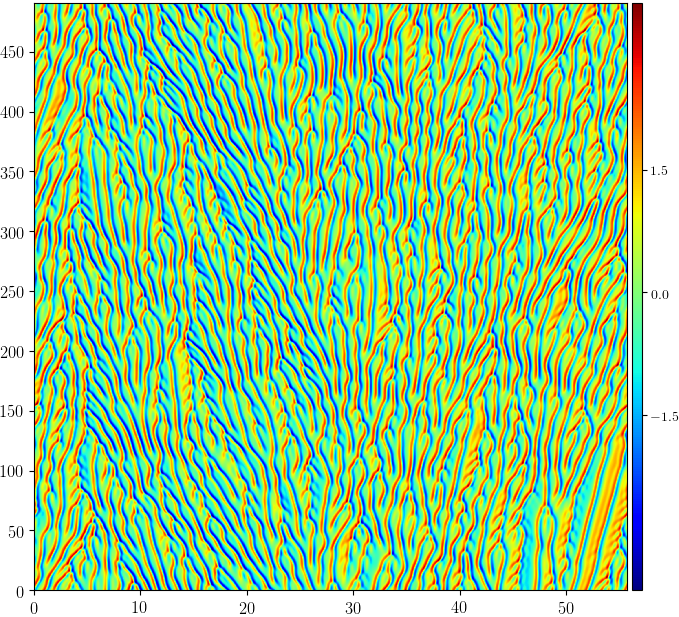
\includegraphics[width=0.9\textwidth]{MNG_u_largeL}
\end{center}
\caption{
A typical {\spt} ``steady state turbulence'' \KS\ solution $u(x,t)$,
integrated forward in time on a periodic domain of size
$\speriod{}\approx 79.57$
(after the initial transient has died out).
The most unstable wavelength $2\pi\sqrt{2}$ of the u=0 \eqv\ (see
\refsect{sect:KSu0equiT}) is an estimate the mean spatial wavelength of
the turbulent \KS\ flow, so there are approximately 55 wiggles across the
spatial domain at any instant in time.
The color bar indicates the color scheme for $u(x,t)$, used also
for the subsequent figures of this type.
     } \label{f:ks_largeL}
\end{figure}

It suffices to inspect a single generic \spt\ solution of \KSe\, such as
\reffig{f:ks_largeL}, to be almost always able to recognize any other solution $u$ as
a solution of \KSe.
Indeed, the goal of this paper is to explain \emph{why}, by deriving the
alphabet of admissible patterns from the \KSe, and assigning a unique
{\spt} ``word'' to any solution that can be seen embedded into
the chaotic (turbulent) attractor (inertial manifold).
It is intuitive by inspection that there is a typical spatial ``mean
wavelength'' (\refsect{sect:KSu0equiT}) and a typical time scale, that
the patterns are exponentially decorrelated beyond several space and time
scale units (\refsect{exam:KurSivTempstab} and \refsect{sect:KSu0equiS}),
and that all statistical averages, such as energies
and dissipation rates, should be extensive (see \refsect{sect:KSenerg}).
